%%%%%%%%%%%%%%%%%%%%%%%%%%%%%%%%%%%%%%%%%%%%%%%%%%%%%
%                                                   %
%     Penn State Colloquium Poster Template         %
%                                                   %
% Uses Penn State Colloquium class, with options:   %
%                                                   %
% Orientation:                                      %
%     portrait (default), landscape                 %
%                                                   %
% Paper size:                                       %
%     a4paper (default), a0paper, a1paper, a2paper, %
%     a3paper, a5paper, a6paper                     %
%%%%%%%%%%%%%%%%%%%%%%%%%%%%%%%%%%%%%%%%%%%%%%%%%%%%%
\documentclass{../psuposter}
\renewcommand{\templateimagepath}{../} 


%%%%%%%%%%%%%%%%%%%%%%%%%%%%%%%%%%%%%%%%%%%%%%%%%%%%%
%               Package Dependencies                %
%%%%%%%%%%%%%%%%%%%%%%%%%%%%%%%%%%%%%%%%%%%%%%%%%%%%%
\usepackage{natbib}
\usepackage{lipsum}                                % Dummy text
\usepackage[figwidth = 0.98\linewidth]{todonotes}  % Dummy image (and more!)
\usepackage[absolute, overlay]{textpos}            % Figure placement
\setlength{\TPHorizModule}{\paperwidth}
\setlength{\TPVertModule}{\paperheight}
\setcitestyle{numbers,square}


%%%%%%%%%%%%%%%%%%%%%%%%%%%%%%%%%%%%%%%%%%%%%%%%%%%%%
%                 AUTHOR AND TITLE                  %
%%%%%%%%%%%%%%%%%%%%%%%%%%%%%%%%%%%%%%%%%%%%%%%%%%%%%
\title{Metal halide perovskites: a frontier material for photovoltaics and advanced semiconductor technologies}
\author{Joseph J. Berry}
\institute{National Renewable Energy Laboratory, Golden, Colorado}


%%%%%%%%%%%%%%%%%%%%%%%%%%%%%%%%%%%%%%%%%%%%%%%%%%%%%
%                  BEGIN DOCUMENT                   %
%%%%%%%%%%%%%%%%%%%%%%%%%%%%%%%%%%%%%%%%%%%%%%%%%%%%%
\begin{document}
\begin{frame}
\begin{columns}[t, totalwidth=\textwidth]
\begin{column}{0.45\textwidth - 1cm}


%%%%%%%%%%%%%%%%%%%%%%%%%%%%%%%%%%%%%%%%%%%%%%%%%%%%%
%                 BLOCK: BIOGRAPHY                  %
%%%%%%%%%%%%%%%%%%%%%%%%%%%%%%%%%%%%%%%%%%%%%%%%%%%%%
    \begin{block}{Speaker Biographic Summary}
    	\begin{center}
    		
\includegraphics[width=0.5\textwidth]{images/berry}
    	\end{center}
    	\href{https://www.nrel.gov/research/staff/joseph-berry.html}{Joseph J. Berry} is a senior research scientist at NREL. He received his PhD in physics from Penn State University in 2001. His thesis work focused on semiconductor spintronics with an emphasis on coherent spin transport across interfaces, spin polarized transport in 2-DEGs, and development of hybrid ferromagnetic semiconductor materials. 
    	%Much of this work is foundational to efforts in the field of spintronics. 
    	From 2001 to 2007, he worked as a postdoctoral researcher at the National Institute of Standards and Technology in Boulder, Colorado.
    	%, specializing in development and application of narrow band spectroscopies to the studies of III-V quantum dots. 
    	From 2007 to the present, Berry has worked as a scientist at NREL on oxide semiconductor systems with a focus on both basic materials physics and device applications of these materials. Berry is also an affiliate of the Renewable and Sustainable Energy Institute and a lecturer in the Department of Physics at the University of Colorado at Boulder.
    \end{block}


%%%%%%%%%%%%%%%%%%%%%%%%%%%%%%%%%%%%%%%%%%%%%%%%%%%%%
%            BLOCK: RESEARCH INTERESTS              %
%%%%%%%%%%%%%%%%%%%%%%%%%%%%%%%%%%%%%%%%%%%%%%%%%%%%%
    \begin{block}{Research Interests}
        Dr. Berry's research on transport at semiconductor interfaces has resulted in significant contributions to advances in organic optoelectronic devices, as well as emerging next-generation photoconversion technologies. Understanding semiconductor structure and its relationship to optoelectronic properties at heterointerfaces is an ongoing theme of his work throughout his scientific carrier. These interests in fundamental aspects of interfaces have also led to ongoing internal and external collaborations to develop solution-processed materials systems, and closely related efforts on high-throughput approaches to material and device development.
        \begin{center}
	    	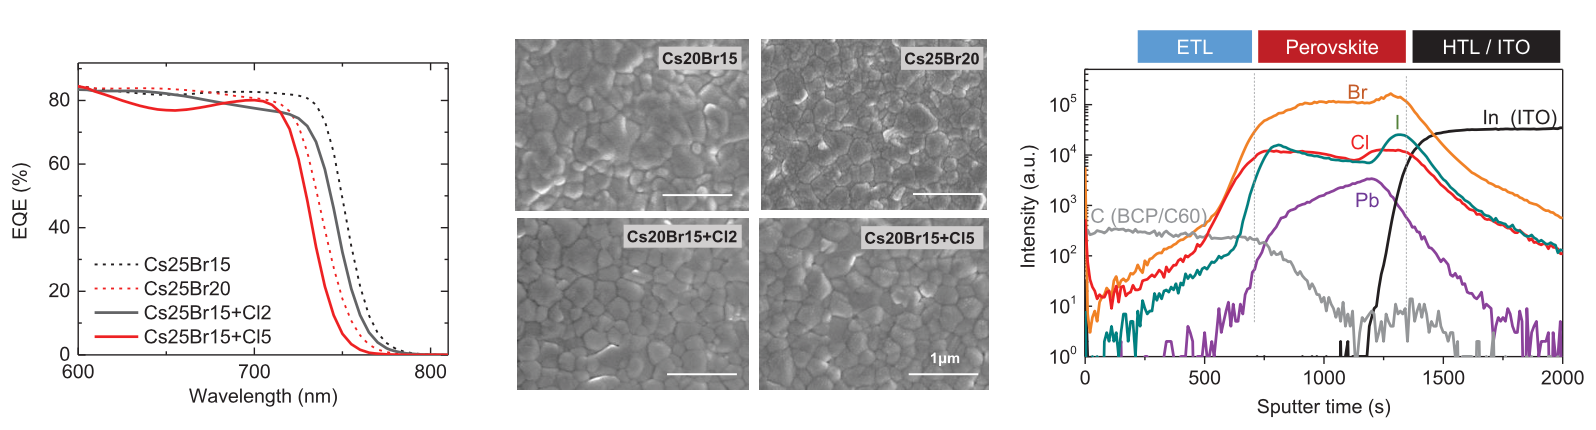
\includegraphics[width=0.85\textwidth]{images/alloy-characteristics}    		
    	\end{center}
    	\textit{Characteristics of triple-halide perovskite alloys}. \cite{xuTriplehalideWideBand2020}
    \end{block}
\end{column}
\begin{column}{0.55\textwidth - 1cm}


%%%%%%%%%%%%%%%%%%%%%%%%%%%%%%%%%%%%%%%%%%%%%%%%%%%%%
%                 BLOCK: ABSTRACT                   %
%%%%%%%%%%%%%%%%%%%%%%%%%%%%%%%%%%%%%%%%%%%%%%%%%%%%%
    \begin{block}{Talk Abstract}
        Metal halide perovskites, particularly the organic-inorganic hybrids are attracting enormous interest as novel semiconductors with excellent performance as photovoltaic devices.  The materials have a number of interesting physical properties that are distinct from traditional inorganic or organic semiconductors. These properties have led to metal halide perovskites showing outstanding performance as photovoltaics, surpassing power conversion efficiency of over 25\% for lab cells and in excess of 18\% for large area devices. This talk will highlight the latest work at NREL to develop a fundamental understanding of the critical roadblocks to implementing metal halide perovskites in next generation photovoltaic applications, including their stability, solar cell performance, device architectures, and operational dynamics. We will also discuss applications beyond photovoltaics in emerging semiconductor technologies. 
    \end{block}


%%%%%%%%%%%%%%%%%%%%%%%%%%%%%%%%%%%%%%%%%%%%%%%%%%%%%
%                BLOCK: BACKGROUND                  %
%%%%%%%%%%%%%%%%%%%%%%%%%%%%%%%%%%%%%%%%%%%%%%%%%%%%%
    \begin{block}{Brief Background}
        Perovskite photovoltaic (PV) technology relies on materials with a particular crystalline structure, similar to that of the mineral perovskite (below, left) \cite{luPerovskiteSolarCells}. These materials are used as the light-harvesting layer of the PV solar cell. Long-term stability of these devices has been the primary obstacle preventing commercialization; however, recent advancements have produced devices with modified architectures that can retain 94\% of peak efficiency over a period of 1,000 hours (below, right). \cite{christiansTailoredInterfacesUnencapsulated2018}
		
        \begin{center}
		   	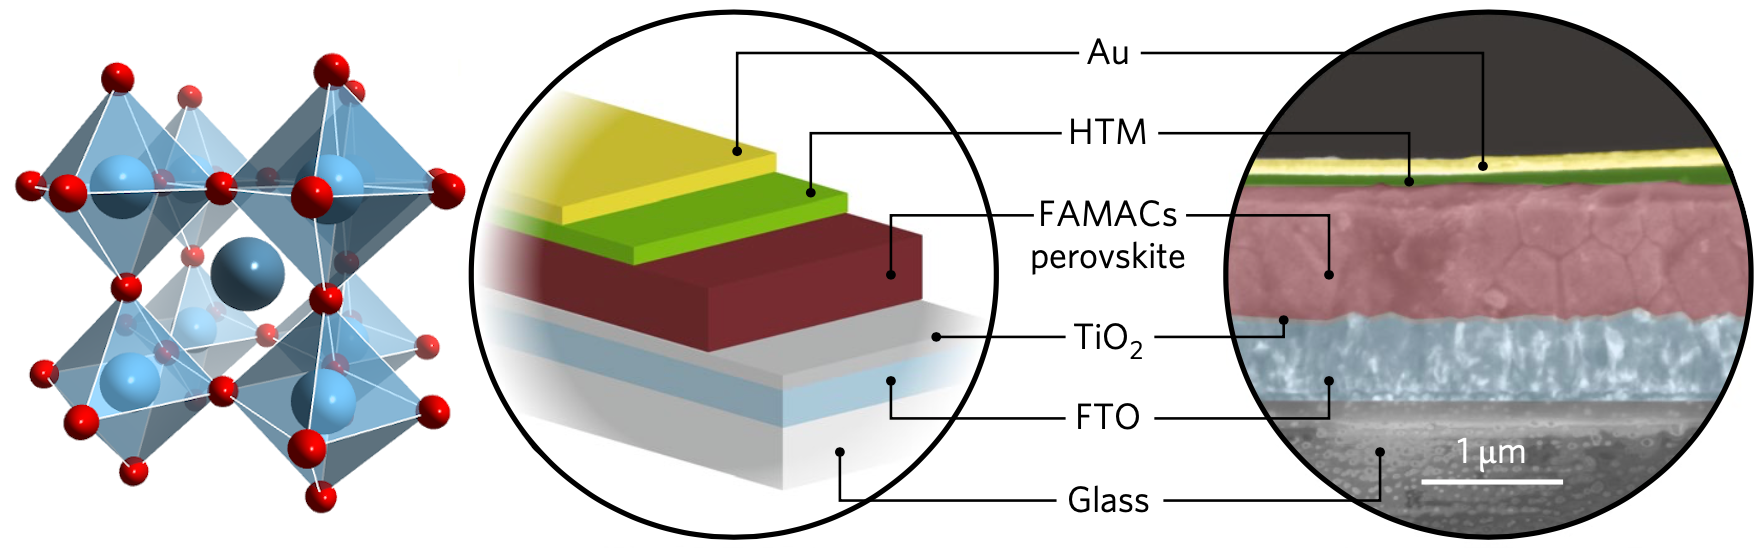
\includegraphics[width=0.9\textwidth]{images/solar-cell}    		
    	\end{center}

		PV technology also presents promising power conversion efficiency (PCE), holding the present record for single-junction devices around 25\%. In order to exceed the thermodynamic single-cell limit, which is the maximum theoretical efficiency of a solar cell using a single p-n junction, more junctions can be added. These ``tandem'' cells represent one of the most promising approaches to surpassing the limit, such as combining a perovskite top cell in tandem with a Si bottom cell. Dr. Berry and team used anion engineering techniques to develop a tandem, wide-bandgap solar cell with 26.7\% PCE. \cite{kimEfficientStableSilicon2020} 

    \end{block}


%%%%%%%%%%%%%%%%%%%%%%%%%%%%%%%%%%%%%%%%%%%%%%%%%%%%%
%                 BLOCK: REFERENCES                 %
%%%%%%%%%%%%%%%%%%%%%%%%%%%%%%%%%%%%%%%%%%%%%%%%%%%%%
    \begin{block}{References}
        \bibliographystyle{aipnum4-1}
%        \bibliographystyle{iopart-num}
		\bibliography{../references}
    \end{block}

\end{column}
\end{columns}


%%%%%%%%%%%%%%%%%%%%%%%%%%%%%%%%%%%%%%%%%%%%%%%%%%%%%
%                    FOOTER TEXT                    %
%%%%%%%%%%%%%%%%%%%%%%%%%%%%%%%%%%%%%%%%%%%%%%%%%%%%%
\begin{textblock}{0.5}(0.18, 0.94)
    \color{white}
    \sffamily
    \textbf{Eberly College of Science}
    \\
    Department of Physics
\end{textblock}


%%%%%%%%%%%%%%%%%%%%%%%%%%%%%%%%%%%%%%%%%%%%%%%%%%%%%
%                   END TEMPLATE                    %
%%%%%%%%%%%%%%%%%%%%%%%%%%%%%%%%%%%%%%%%%%%%%%%%%%%%%
\end{frame}
\end{document}
